\documentclass[preview]{standalone}

\usepackage{amsmath}
\usepackage{amssymb}
\usepackage{parskip}
\usepackage{fullpage}
\usepackage{hyperref}
\usepackage{tikz}
\usepackage{wrapfig}
\usepackage{bettelini}
\usepackage{stellar}

\hypersetup{
    colorlinks=true,
    linkcolor=black,
    urlcolor=blue,
    pdftitle={Theory of Computation},
    pdfpagemode=FullScreen,
}

% =======
\usetikzlibrary{ % tikz packages
    automata,positioning,
    arrows.meta,bending
}
\tikzset{every state/.style={
    inner sep=2pt,
    minimum size=4pt
}}
\tikzset{>=stealth}  %latex, to, stealth
% Empty string symbol.
\newcommand{\emptyString}{\lambda}
% =======

\begin{document}

\title{Theory of Computation}
\id{theoryofcomputation-regular-languages}
\genpage

\section{Regular languages}

\begin{snippetdefinition}{regular-language-definition}{Regular language}
    A language \(A\) is \textit{regular} if there exists an automaton \(M\) that accepts it.
    \[
        \exists M \suchthat L(M) = A
    \]
\end{snippetdefinition}

\section{Closure under union (extra)}

\plain{The following proof is extra because we will prove a stronger result using NFAs.}

\begin{snippetproposition}{closure-under-union-using-dfa}{Closure under union}
    \textit{If \(A\) and \(B\) are two regular languages over the same alphabet
    \(\Sigma\), then \(A \union B\) is also regular.}
\end{snippetproposition}

\begin{snippetproof}{closure-under-union-using-dfa-proof}{Closure under union}
    We can prove this by making a DFA that accepts both languages.
    Let \(M_1=(Q_1, \Sigma, \delta_1, q_1, F_1)\) be a DFA that accepts \(A\)
    and \(M_2=(Q_2, \Sigma, \delta_2, q_2, F_2)\) an automaton that accepts \(B\).
    The automaton \(M=(Q, \Sigma, \delta, q, F)\) must run \(M_1\) and \(M_2\) \textit{simultaneously},
    so any state must represent the current states of \(M_1\) and \(M_2\).
    This means that the states of \(M\) must represent any combination of state between
    \(M_1\) and \(M_2\), meaning \(Q=Q_1 \times Q_2\).
    The transition function is now in the form
    \(\delta((r_1, r_2), a) = (\delta_1(r_1, a), \delta_2(r_2, a))\) where \(a\in\Sigma\).
    The initial state is the state in \(Q\) which contains the initial state of \(M_1\)
    and \(M_2\), namely \((q_1, q_2)\). Finally, the set of accept states
    is every tuple in \(Q_1\) containing a state in \(F_2\) or in \(Q_2\) containing a state in \(F_1\), namely
    \(Q_1 \times F_2 \union Q_2 \times F_1\). \\
    We can conclude that \(M=(Q_1 \times Q_2, \Sigma, \delta((r_1, r_2), a), (q_1, q_2), Q_1 \times F_2 \union Q_2 \times F_1)\)
    accepts \(A \union B\) so \(A \union B\) is regular.
\end{snippetproof}


\section{Closure under regular operations}

\begin{snippettheorem}{nfa-closure-under-regular-operations}{NFA closure under regular operations}
    Let \(A\) and \(B\) be two regular languages over \(\Sigma\).
    Then, the following languages:
        \(A \union B\),
        \(AB\),
        \(A^*\),
        \(\bar{A}\) and
        \(A \intersection B\)
    are also regular.
\end{snippettheorem}

\begin{snippetproof}{nfa-closure-under-regular-operations-proof}{NFA closure under regular operations}
    \begin{enumerate}
        \item \textbf{closure under union:}
        Let \(N_1 = (Q_1, \Sigma, \delta_1, q_1, F_1)\) and
        \(N_2 = (Q_2, \Sigma, \delta_2, q_2, F_2)\) be two NFAs such that
        \(A_1 = L(N_1)\) and \(A_2 = L(N_2)\).
        We can construct another NFA \(N=(Q, \Sigma, \delta, q_0, F)\)
        such that \(L(N)=A\union B\).
        \(N\) will either go to \(N_1\) or \(N_2\) by making a \(\emptyString\)-transition.
        \begin{itemize}
            \item \(Q=\{q_0\} \union Q_1 \union Q_2\)
            \item \(F=F_1 \union F_2\)
            \item \[
                \delta(r, a) =
                \begin{cases}
                    \delta_1(r, a) & r \in Q_1 \\
                    \delta_2(r, a) & r \in Q_2 \\
                    \{q_1, q_2\} & r = \emptyString \\
                    \emptyset & r \neq \emptyString
                \end{cases}
            \]
        \end{itemize}
        
        \begin{center}
            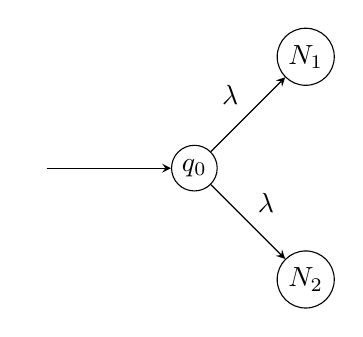
\begin{tikzpicture}[node distance=2cm,on grid,auto]
                \node[state] (0) {\(q_0\)};
                \node (inv) [left=of 0] {};
        
                \node[state] (a1) [above right=of 0] {\(N_1\)};
                
                \node[state] (b1) [below right=of 0] {\(N_2\)};
                
                \path[->]
                    (inv)
                        edge node {} (0)
                    (0)
                        edge node {\(\emptyString\)} (a1)
                        edge node {\(\emptyString\)} (b1);
            \end{tikzpicture}
        \end{center}
        \item \textbf{closure under concatenation:}
        Let \(N_1 = (Q_1, \Sigma, \delta_1, q_1, F_1)\) and
        \(N_2 = (Q_2, \Sigma, \delta_2, q_2, F_2)\) be two NFAs such that
        \(A_1 = L(N_1)\) and \(A_2 = L(N_2)\).
        We can construct another NFA \(N=(Q, \Sigma, \delta, q_0, F)\)
        such that \(L(N)=AB\).
        \(N\) will start by executing \(N_1\), meaning \(q_0=q_1\). If \(N\) switches to a state
        \(r\in F_1\) it can move to executing \(N_2\) with a \(\emptyString\)-transition.
        The accepted states are only the ones of \(N_2\) meaning \(F=F_2\). \(Q=Q_1 \union Q_2\).
        The transition function is hence defined as
        \[
            \delta(r, a)
            \begin{cases}
                \delta_1(r, a) & (r \in Q_1 \land r \notin F_1) \lor (r \in F_1 \land r \neq \emptyString) \\
                \delta_1(r, a) \union \{q_2\} & r \in F_1 \land r = \emptyString \\
                \delta_2(r, a) & r \in Q_2
            \end{cases}
        \]
        
        \begin{center}
            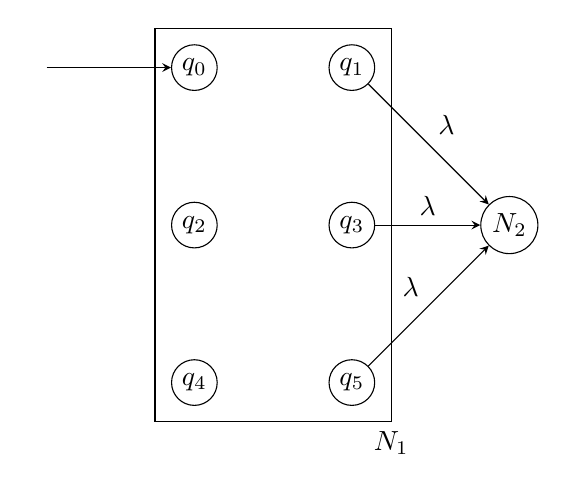
\begin{tikzpicture}[node distance=2cm,on grid,auto]
                \node[state] (q0) {\(q_0\)};
                \node (inv) [left=of q0] {};
        
                \node[state] (q1) [right=of q0] {\(q_1\)};
                \node[state] (q2) [below=of q0] {\(q_2\)};
                \node[state] (q3) [below=of q1] {\(q_3\)};
                \node[state] (q4) [below=of q2] {\(q_4\)};
                \node[state] (q5) [below=of q3] {\(q_5\)};
        
                \node[state] (n2) [right=of q3] {\(N_2\)};
        
                \draw[draw=black] (q0) ++(-0.5, 0.5) rectangle ++(3,-5) node[below] {\(N_1\)};
        
                \path[->]
                    (inv)
                        edge node {} (q0)
                    (q1)
                        edge node {\(\emptyString\)} (n2)
                    (q3)
                        edge node {\(\emptyString\)} (n2)
                    (q5)
                        edge node {\(\emptyString\)} (n2);
            \end{tikzpicture}
        \end{center}
        Here \(F_1 = \{q_1, q_3, q_5\}\) but the actual accept states are the ones for \(N_2\).
        \item \textbf{closure under Kleene star:}
        Let \(N_1 = (Q_1, \Sigma, \delta_1, q_0, F_1)\) be a NFAs such that
        \(A_1 = L(N_1)\). We can construct another NFA \(N=(Q, \Sigma, \delta, q, F)\)
        such that \(L(N)=A_1^*\).
        We want \(N_1\) to be able to switch back to its initial point
        when it is in a state \(r \in F_1\). This means that the concatenation of
        accepted strings can cycle one after the other. Since \(\emptyString\)
        also needs to be accepted we need a new start state which is an accept state.
        
        \begin{itemize}
            \item \(Q = \{q_a\} \union Q_1\)
            \item \(q = q_a\)
            \item \(F = F_1 \union \{q\}\)
            \item \[
                \delta(r,a) =
                \begin{cases}
                    \delta_1(r,a) & (r \in Q_1 \land r \notin F_1) \lor (r \in F_1 \land a \neq \emptyString) \\
                    \delta_1(r,a) \union \{q_0\} & r \in F_1 \land a = \emptyString \\
                    \{q_0\} & r = q \land a = \emptyString \\
                    \emptyset & r = q \land a \neq \emptyString
                \end{cases}
            \]
        \end{itemize}
        
        \begin{center}
            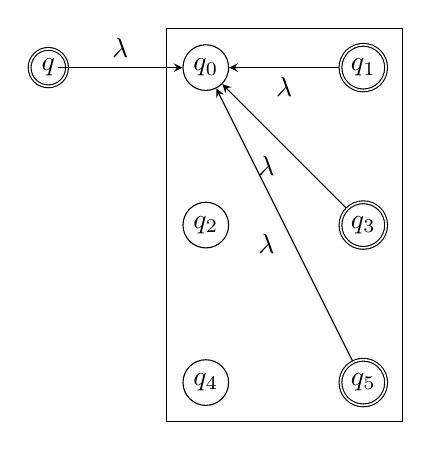
\begin{tikzpicture}[node distance=2cm,on grid,auto]
                \node[state, accepting] (q) {\(q\)};
                \node[state] (q0) [right=of q] {\(q_0\)};
                \node (inv) [left=of q0] {};
        
                \node[state, accepting] (q1) [right=of q0] {\(q_1\)};
                \node[state] (q2) [below=of q0] {\(q_2\)};
                \node[state, accepting] (q3) [below=of q1] {\(q_3\)};
                \node[state] (q4) [below=of q2] {\(q_4\)};
                \node[state, accepting] (q5) [below=of q3] {\(q_5\)};
        
                \draw[draw=black] (q0) ++(-0.5, 0.5) rectangle ++(3,-5);
        
                \path[->]
                    (inv)
                        edge node {\(\emptyString\)} (q0)
                    (q1)
                        edge node {\(\emptyString\)} (q0)
                    (q3)
                        edge node {\(\emptyString\)} (q0)
                    (q5)
                        edge node {\(\emptyString\)} (q0);
            \end{tikzpicture}
        \end{center}
        \item \textbf{closure under complement:}
        Let \(N_1 = (Q_1, \Sigma, \delta_1, q_0, F_1)\) be a NFAs such that
        \(A_1 = L(N_1)\). We can construct another NFA \(N=(Q, \Sigma, \delta, q, F)\)
        such that \(L(N)=\bar{A_1}\).
        Any state \(r \notin F_1\) will be able to switch to a new state \(q_a\),
        which is the only accept state of \(N\), with a \(\emptyString\)-transition.
        This will negate any accepting state of \(N_1\) and vice versa.
        
        \begin{itemize}
            \item \(Q=\{q_a\} \union Q_1\)
            \item \(q = q_0\)
            \item \(F = \{q_a\}\)
            \item \[
                \delta(r,a) =
                \begin{cases}
                    \delta_1(r,a) \union \{q_a\} & r \in F_1 \\
                    \delta_1(r,a) & r \notin F_1 \\
                \end{cases}
            \]
        \end{itemize}
        
        \begin{center}
            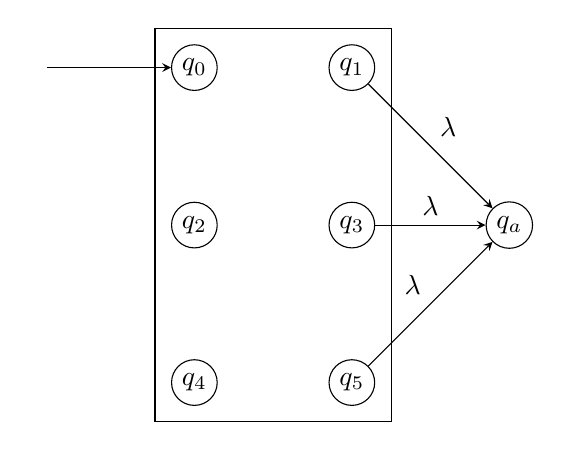
\begin{tikzpicture}[node distance=2cm,on grid,auto]
                \node[state] (q0) {\(q_0\)};
                \node (inv) [left=of q0] {};
        
                \node[state] (q1) [right=of q0] {\(q_1\)};
                \node[state] (q2) [below=of q0] {\(q_2\)};
                \node[state] (q3) [below=of q1] {\(q_3\)};
                \node[state] (q4) [below=of q2] {\(q_4\)};
                \node[state] (q5) [below=of q3] {\(q_5\)};
        
                \node[state] (n2) [right=of q3] {\(q_a\)};
        
                \draw[draw=black] (q0) ++(-0.5, 0.5) rectangle ++(3,-5);
        
                \path[->]
                    (inv)
                        edge node {} (q0)
                    (q1)
                        edge node {\(\emptyString\)} (n2)
                    (q3)
                        edge node {\(\emptyString\)} (n2)
                    (q5)
                        edge node {\(\emptyString\)} (n2);
            \end{tikzpicture}
        \end{center}
        Here \(F_1=\{q_0, q_2, q_4\}\), but the only actual accept state is \(q_a\).
        \item \textbf{closure under intersection:}
        Since \(A\union B\) is regular and \(A \intersection B \subseteq A \union B\),
        \(A \intersection B\) is also regular.
    \end{enumerate}
\end{snippetproof}

\end{document}